\svnInfo $Id$

ICON output fields are exclusively available in GRIB2 format (\textbf{GRI}dded \textbf{B}inary Edition \textbf{2}), with the exception of 
meteogram data (NetCDF). GRIB is a bit-oriented data storage format which was developed by \gls{WMO} to facilitate the exchange of large volumes of 
gridded data between weather prediction centres. For decoding and encoding GRIB2 messages, the DWD in general and ICON in particular 
makes use of the ECMWF GRIB API. The current operational version at DWD is $1.13.1$.
 
In GRIB2, a product (i.e.\ a variable/field) is identified by a set of three parameters
% variable is uniquely defined by the following set of metadata:
\begin{itemize}
 \item \emph{Discipline} (see GRIB2 code table 0.0)
 \item \emph{ParameterCategory} (see GRIB2 code table 4.1)
 \item \emph{ParameterNumber} (see GRIB2 code table 4.2), 
\end{itemize}
augmented by a large number of additional metadata in order to uniquely describe the nature of the data. Noteworthy examples 
of additional metadata are 
\begin{itemize}
  \item \emph{typeOfFirstfixedSurface} and \emph{typeOfSecondFixedSurface} (see GRIB2 code table 4.5)
  \item \emph{typeOfStatisticalProcessing}, former known as \emph{stepType} (instant, accum, avg, max, min, diff, rms, sd, cov, \dots),
        describing the statistical process used to calculate the field
 \end{itemize}
just to name a few.

A documentation of the official WMO GRIB2 code tables can be found here: 

\begin{minipage}{\textwidth}
\url{http://www.wmo.int/pages/prog/www/WMOCodes/WMO306_vI2/LatestVERSION/WMO306_vI2_GRIB2_CodeFlag_en.pdf}
\end{minipage}

In the following tables \emph{typeOfFirstFixedSurface} and \emph{typeOfSecondFixedSurface} will be abbreviated by \emph{Lev-Typ~1/2}.



% --------------------------------------------------------------------------------
\section{Deprecated output fields}
% --------------------------------------------------------------------------------

With the launch of ICON, the following former GME output fields are no longer available:

\begin{itemize}
 \item \textbf{BAS\_CON} [\textendash]: Level index of convective cloud base. Instead, \textbf{HBAS\_CON} [m] should be used.
 \item \textbf{TOP\_CON} [\textendash]: Level index of convective cloud top. Instead, \textbf{HTOP\_CON} [m] should be used.
 \item \textbf{W\_G1}, \textbf{W\_G2}  [mm H2O]: Soil water content in upper layer ($0$ to $10\,\mathrm{cm}$) and middle layer ($10$ to $100\,\mathrm{cm}$), respectively. 
                                                 If needed, these fields can be derived from \textbf{W\_SO}.
 \item \textbf{FIS} [$\mathrm{m^{2}\,s^{-1}}$]: Surface Geopotential. Instead, \textbf{HSURF} $[\mathrm{m}]$ should be used (see Section \ref{sec_newout}).
 \item \textbf{O3} [$\mathrm{kg/kg}$], \textbf{TO3} [$\mathrm{Dobson}$]: Ozone mixing ratio and corresponding total ozone concentration. No longer available; no substitution
\end{itemize}


% --------------------------------------------------------------------------------
\section{New output fields}\label{sec_newout}
% --------------------------------------------------------------------------------

Table \ref{table_newout} contains a list of new output fields that became available with the launch of ICON (compared to GME). A more thorough description of these 
fields is provided in Section \ref{sec_outfields}.
\begin{longtable}{p{2.5cm}p{1.8cm}p{10.0cm}}
 \captionabove{Newly available output fields}\label{table_newout}\\
  \toprule
\multicolumn{1}{c}{\textbf{ShortName}}  &  \bf{Unit}                  & \multicolumn{1}{c}{\textbf{Description}}\\
\midrule
\endfirsthead
\caption[]{\emph{continued}}\\
\midrule
\endhead
\hline \multicolumn{3}{r}{\textit{Continued on next page}} \\
\endfoot
\endlastfoot
\midrule
\multicolumn{3}{c}{\textbf{Atmosphere}}\\
\midrule
\textbf{DEN}                            &  $\mathrm{kg\,m^{-3}}$      &  Density of moist air (3D field) \\
\textbf{TKE}                            &  $\mathrm{m^{2}\,s^{-2}}$   &  Turbulent kinetic energy (3D field) \\
\textbf{DTKE\_CON}                      &  $\mathrm{m^{2}\,s^{-3}}$   &  Buoyancy-production of TKE due to sub grid scale convection (3D field) \\
\textbf{DTKE\_HSH}                      &  $\mathrm{m^{2}\,s^{-3}}$   &  Production of TKE due to horizontal shear (3D field) \\
\textbf{W}                              &  $\mathrm{m\,s^{-1}}$       &  Vertical velocity in height coordinates $w=\frac{\mathrm{d}z}{\mathrm{d}t}$ (3D field)\\
\textbf{P}                              &  $\mathrm{Pa}$              &  Pressure (3D field)\\
\midrule
\multicolumn{3}{c}{\textbf{Surface}}\\
\midrule
\textbf{CAPE\_CON}                      &  $\mathrm{J\,kg^{-1}}$      &  Convective available potential energy (2D field) \\
\textbf{QV\_2M}                         &  $\mathrm{kg\, kg^{-1}}$    &  Specific humidity at 2m above ground (2D field) \\
\textbf{RELHUM\_2M}                     &  $\mathrm{\%}$              &  Relative humidity at 2m above ground (2D field) \\
\textbf{SOBS\_RAD}                      &  $\mathrm{W\,m^{-2}}$       &  Net short-wave radiation flux at surface (instantaneous) \\
\textbf{THBS\_RAD}                      &  $\mathrm{W\,m^{-2}}$       &  Net long-wave radiation flux at surface (instantaneous) \\
%
\midrule
\multicolumn{3}{c}{\textbf{Lake}}\\
\midrule
\textbf{C\_T\_LK}                       &  $1$                        &  Shape factor with respect to the temperature profile in the thermocline (2D field)\\
\textbf{H\_ML\_LK}                      &  $\mathrm{m}$               &  Mixed-layer depth (2D field)\\
\textbf{T\_BOT\_LK}                     &  $\mathrm{K}$               &  Temperature at the water-bottom sediment interface (2D field)\\
\textbf{T\_MNW\_LK}                     &  $\mathrm{K}$               &  Mean temperature of the water column (2D field)\\
\textbf{T\_WML\_LK}                     &  $\mathrm{K}$               &  Mixed-layer temperature (2D field)\\
\midrule
\multicolumn{3}{c}{\textbf{Geometry}}\\
\midrule
\textbf{HSURF}                          &  $\mathrm{m}$               &  Geometric Height of the earths surface above sea level (2D field) \\
\textbf{HHL}                            &  $\mathrm{m}$               &  Geometric Height of model half levels above sea level (3D field) \\
\textbf{CLON,CLAT}                      &  $\mathrm{deg}$             &  Geographical longitude/latitude of native grid triangle cell center \\
\textbf{ELON,ELAT}                      &  $\mathrm{deg}$             &  Geographical longitude/latitude of native grid triangle edge midpoint \\
  \bottomrule
\end{longtable}


% --------------------------------------------------------------------------------
\section{Available output fields}\label{sec_outfields}
% --------------------------------------------------------------------------------

ICON forecasts are performed multiple times a day with varying forecast periods. An overview of the forecast runs, including its  
forecast period and output intervals is provided in Figure \ref{fig:forecast_length_global}.
\begin{figure}[hbt]
 \centering
 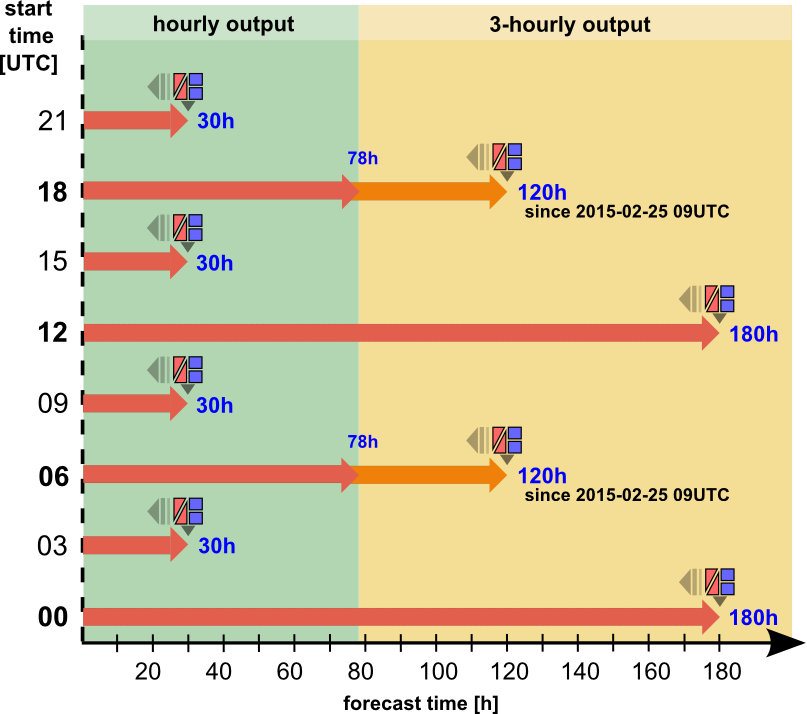
\includegraphics[width=0.90\textwidth]{forecast_length_global.png}
 \caption{Time span covered by the various global ICON forecasts which are launched every three hours.
          Output on the native (triangular) grid (\protect\markRed) and the regular grid (\protect\markBlue) 
          is generally available until forecast end, as indicated by the lenght of the two bars shown for 
          each forecast run. Output fields are available hourly up to $VV=78\,\mathrm{h}$ and 3-hourly for 
          larger forecast times.}\label{fig:forecast_length_global}
\end{figure}

Main forecasts are performed $4$ times a day at $0,\, 6,\, 12,\, 18$ UTC, covering a forecast time span of $180\,\mathrm{h}$ for the 
$0$ und $12$ UTC runs and $120\,\mathrm{h}$ for the $6$ und $18$ UTC runs. Prior to 2015-02-25 the 6 and 18 UTC runs were restricted 
to $78\,\mathrm{h}$. In preparation for the replacement of COSMO-EU by a high resolution ICON nest, additional short-range forecasts 
are performed at 3, 9, 15 and 21UTC. The ICON nest will provide boundary data for the high resolution COSMO-DE runs, once COSMO-EU has 
been switched off later this year. The forecast time covered by these runs is limited to $30\,\mathrm{h}$. See Chapter 
\ref{nest:chap_forecast_runs} for more details on the ICON nest and the available output fields. 

All time-dependent output fields are available hourly up to
$VV=78\,\mathrm{h}$ and 3-hourly for larger forecast
times\footnotemark[2].
%
Please note that for ICON fields the time unit is minutes rather than
hours, and thus differs from GME (hours).

Output is available on two distinct horizontal grids: 
\begin{itemize}
  \item The native triangular grid with an average resolution of $13\,\mathrm{km}$, and
  \item a regular latitude-longitude grid with a resolution of $\Delta \lambda = \Delta \Phi=0.25^{\circ}$. 
\end{itemize}
On the native grid most output fields are defined on triangle cell
(circum-)centers, except for \texttt{VN}, which is defined on cell
edges. On the lat-lon grid, all fields are defined on cell centers.
%
A single 2D GRIB2 field on the native and regular lat-lon grid
contains $2949120$ and $1038240$ ($721 \times 1440$) grid points, respectively.


For details regarding the available fields, please see the tables below. Note that the vertical rules in the leftmost column indicate whether the field is 
available on the native grid ($\,$\markRed$\,$), on the lat-lon grid($\,$\markBlue$\,$), or on both grids($\,$\markRed\markBlue$\,$). 

For details regarding the algorithm for interpolation onto the lat-lon
grid, see
Section~\ref{section:technical_details_of_the_horizontal_interpolation}. In the tables below, the specific algorithm used for 
lat-lon interpolation is indicated in the column \texttt{LL IntpType}. If nothing is specified, then an RBF-based interpolation 
method is used.

\footnotetext[2]{An exception here are the output fields \texttt{VMAX\_10M}, \texttt{U\_10M} and \texttt{V\_10M}, 
which are available hourly throughout the forecast. For the latter two this is because \texttt{U\_10M} and \texttt{V\_10M} 
are needed as input by the wave models.}


% --------------------------------------------------------------------------------
\subsection{Time-constant (external parameter) fields}\label{sec_const_outfields}
% --------------------------------------------------------------------------------

Table \ref{table_constdb} provides an overview of the available time invariant fields. They are available from the database category 
\texttt{CAT\_NAME=\$model\_\tblu{const}\_\tblu{an}\_\$suite}. As mentioned in Section \ref{section:extpar}, \texttt{DEPTH\_LK}, 
\texttt{HSURF}, \texttt{FR\_LAND}, \texttt{FR\_LAKE} and \texttt{Z0} are modified by ICON. Thus, the latter should 
not be taken from the \emph{const\_an} database category, unless you definitely know what you are doing. For convenience, the 
modified invariant fields (and some more) are stored in the \emph{forecast} database categories for step $s[h]=0$ 
(\texttt{CAT\_NAME=\$model\_\$run\_\tblu{fc}\_\$suite}). Table \ref{table_init_output} provides a list of all fields which are exclusively 
written for $s[h]=0$.

See Section \ref{sec_skycat} for more details on the database categories and Section \ref{sec_example} for sample retrievals.
 

%All except for \texttt{HHL}, \texttt{ELON}, \texttt{ELAT}, 
%\texttt{VLON}, \texttt{VLAT} are available from the database category \texttt{CAT\_NAME=\$model\_\tblu{const}\_\tblu{an}\_\$suite}. However, since  
%\texttt{HSURF}, \texttt{FR\_LAND}, \texttt{FR\_LAKE} and \texttt{Z0} are modified by ICON, they should be taken as well as \texttt{HHL} from 
%\emph{forecast} database categories for step $s[h]=0$ (\texttt{CAT\_NAME=\$model\_\$run\_\tblu{fc}\_\$suite}). See Section 
%\ref{sec_skycat} for more details on the database categories and Section \ref{sec_example} for sample retrievals.

% \begin{vartable}{\caption{Time-constant fields (\texttt{CAT\_NAME=\$model\_\tblu{const}\_\tblu{an}\_\$suite})}\label{table_constdb}}
%     
% \multicolumn{8}{c}{\textbf{Date/Time} (YYYY-MM-DDThh) \textbf{D=0001-01-01T00}}\\
% \midrule
% \groups[tri][]   & CLAT                          &  Geographical latitude of native grid triangle cell center                              &               0                                   &                     191                     &                    1                       &                 1/--                            &                      inst                   &        $\mathrm{Deg.\, N}$   \\
% \groups[tri][]   & CLON                          &  Geographical longitude of native grid triangle cell center                             &               0                                   &                     191                     &                    2                       &                 1/--                            &                      inst                   &        $\mathrm{Deg.\, E}$   \\
% \groups[tri][]   & DEPTH\_LK                     &  Lake depth                                                                             &               1                                   &                       2                     &                    0                       &                 1/162                           &                      inst                   &        $\mathrm{m}$ \\
% \groups[tri][]   & EMIS\_RAD                     &  Longwave surface emissivity                                                            &               2                                   &                       3                     &                  199                       &                 1/--                            &                      inst                   &        $1$ \\
% \groups[tri][]   & FOR\_D                        &  Fraction of deciduous forest (possible range [$0,1$])                                  &               2                                   &                       0                     &                   30                       &                 1/--                            &                      inst                   &        $1$ \\
% \groups[tri][]   & FOR\_E                        &  Fraction of evergreen forest (possible range [$0,1$])                                  &               2                                   &                       0                     &                   29                       &                 1/--                            &                      inst                   &        $1$ \\
% \groups[tri][]   & FR\_LAKE                      &  Fresh water lake fraction (possible range [$0,1$])                                     &               1                                   &                       2                     &                    2                       &                 1/--                            &                      inst                   &        $1$ \\
% \groups[tri][]   & FR\_LAND                      &  Land fraction (possible range [$0,1$])                                                 &               2                                   &                       0                     &                    0                       &                 1/--                            &                      inst                   &        $1$ \\
% \groups[tri][]   & FR\_LUC                       &  Land use class fraction (possible range [$0,1$])                                       &               2                                   &                       0                     &                   36                       &                 1/--                            &                      inst                   &        $1$ \\
% \groups[tri][]   & HSURF                         &  Geometric height of the earths surface above msl                                       &               0                                   &                       3                     &                    6                       &                 1/101                           &                      inst                   &        $\mathrm{m}$   \\ 
% \groups[tri][]   & LAI\_MX                       &  Leaf area index in the vegetation phase                                                &               2                                   &                       0                     &                   28                       &                 1/--                            &                      max                    &        $1$ \\
% \groups[tri][]   & NDVI\_MAX                     &  Normalized differential vegetation index                                               &               2                                   &                       0                     &                   31                       &                 1/--                            &                      max                    &        $1$ \\
% \groups[tri][]   & PLCOV\_MX                     &  Plant covering degree in the vegetation phase                                          &               2                                   &                       0                     &                    4                       &                 1/--                            &                      max                    &        $1$ \\
% \groups[tri][]   & ROOTDP                        &  Root depth of vegetation                                                               &               2                                   &                       0                     &                   32                       &                 1/--                            &                      inst                   &        $\mathrm{m}$ \\
% \groups[tri][]   & RSMIN                         &  Minimum stomatal resistance                                                            &               2                                   &                       0                     &                   16                       &                 1/--                            &                      inst                   &        $\mathrm{s\,m^{-1}}$ \\
% \groups[tri][]   & SOILTYP                       &  Soil type of land fraction  (9 types $[1,\dots, 9]$)                                   &               2                                   &                       3                     &                  196                       &                 1/--                            &                      inst                   &        $1$ \\
% \groups[tri][]   & SSO\_GAMMA                    &  Anisotropy of sub-gridscale orography                                                  &               0                                   &                       3                     &                   24                       &                 1/--                            &                      inst                   &        $1$ \\
% \groups[tri][]   & SSO\_SIGMA                    &  Slope of sub-gridscale orography                                                       &               0                                   &                       3                     &                   22                       &                 1/--                            &                      inst                   &        $1$ \\
% \groups[tri][]   & SSO\_STDH                     &  Standard deviation of sub-grid scale orography                                         &               0                                   &                       3                     &                   20                       &                 1/--                            &                      inst                   &        $\mathrm{m}$ \\
% \groups[tri][]   & SSO\_THETA                    &  Angle of sub-gridscale orography                                                       &               0                                   &                       3                     &                   21                       &                 1/--                            &                      inst                   &        $\mathrm{rad}$ \\
% \groups[tri][]   & T\_2M\_CL                     &  Climatological $2\,\mathrm{m}$ temperature (used as lower bc.\ for soil model)         &               0                                   &                       0                     &                    0                       &               103/--                            &                      inst                   &        $\mathrm{K}$ \\
% \groups[tri][]   & Z0                            &  Surface roughness length (over land)                                                   &               2                                   &                       0                     &                    1                       &                 1/--                            &                      inst                   &        $\mathrm{m}$ \\
% \midrule
% \multicolumn{8}{c}{\textbf{Date/Time} (YYYY-MM-DDThh) \textbf{D=1111-01-11T11}}\\
% \midrule
% \groups[tri][] & AER\_SS12                     &  Sea salt aerosol climatology (monthly fields)                                          &               0                                   &                      20                     &                   102                      &                 1/--                            &                      avg                    &        $\mathrm{1}$ \\
% \groups[tri][] & AER\_DUST12                   &  Total soil dust aerosol climatology (monthly fields)                                   &               0                                   &                      20                     &                   102                      &                 1/--                            &                      avg                    &        $\mathrm{1}$ \\
% \groups[tri][] & AER\_ORG12                    &  Organic aerosol climatology (monthly fields)                                           &               0                                   &                      20                     &                   102                      &                 1/--                            &                      avg                    &        $\mathrm{1}$ \\
% \groups[tri][] & AER\_SO412                    &  Total sulfate aerosol climatology (monthly fields)                                     &               0                                   &                      20                     &                   102                      &                 1/--                            &                      avg                    &        $\mathrm{1}$ \\
% \groups[tri][] & AER\_BC12                     &  Black carbon aerosol climatology (monthly fields)                                      &               0                                   &                      20                     &                   102                      &                 1/--                            &                      avg                    &        $\mathrm{1}$ \\
% \groups[tri][] & ALB\_DIF12                    &  Shortwave ($0.3 - 5.0\,\mathrm{\mu m}$) albedo for diffuse radiation (monthly fields)  &               0                                   &                      19                     &                    18                      &                 1/--                            &                      avg                    &        $\mathrm{1}$ \\
% \groups[tri][] & ALB\_UV12                     &  UV-visible ($0.3 - 0.7\,\mathrm{\mu m}$) albedo for diffuse radiation (monthly fields) &               0                                   &                      19                     &                   222                      &                 1/--                            &                      avg                    &        $\mathrm{1}$ \\
% \groups[tri][] & ALB\_NI12                     &  Near infrared ($0.7 - 5.0\,\mathrm{\mu m}$) albedo for diffuse radiation (monthly fields) &            0                                   &                      19                     &                   223                      &                 1/--                            &                      avg                    &        $\mathrm{1}$ \\
% \groups[tri][] & NDVI\_MRAT                    &  ratio of monthly mean NDVI (normalized differential vegetation index) to annual max    &               0                                   &                       0                     &                   192                      &                 1/--                            &                      avg                    &        $\mathrm{1}$ \\
% 
% \end{vartable}


\begin{vartable}{\captionabove{Time-constant fields (\texttt{CAT\_NAME=\$model\_\tblu{const}\_\tblu{an}\_\$suite})}\label{table_constdb}}
    
\multicolumn{8}{c}{\textbf{Date/Time} (YYYY-MM-DDThh) \textbf{D=0001-01-01T00}}\\
\midrule
\groups[tri][]   & CLAT                          &  Geographical latitude of native grid triangle cell center                              &               0/191/1                             &                 1/--                            &                      inst                   &   --     &    $\mathrm{Deg.\, N}$   \\
\groups[tri][]   & CLON                          &  Geographical longitude of native grid triangle cell center                             &               0/191/2                             &                 1/--                            &                      inst                   &   --     &    $\mathrm{Deg.\, E}$   \\
\groups[tri][]   & DEPTH\_LK                     &  Lake depth                                                                             &               1/2/0                               &                 1/162                           &                      inst                   &   --     &    $\mathrm{m}$ \\
\groups[tri][]   & EMIS\_RAD                     &  Longwave surface emissivity                                                            &               2/3/199                             &                 1/--                            &                      inst                   &   --     &    $1$ \\
\groups[tri][]   & FOR\_D                        &  Fraction of deciduous forest (possible range [$0,1$])                                  &               2/0/30                              &                 1/--                            &                      inst                   &   --     &    $1$ \\
\groups[tri][]   & FOR\_E                        &  Fraction of evergreen forest (possible range [$0,1$])                                  &               2/0/29                              &                 1/--                            &                      inst                   &   --     &    $1$ \\
\groups[tri][]   & FR\_LAKE                      &  Fresh water lake fraction (possible range [$0,1$])                                     &               1/2/2                               &                 1/--                            &                      inst                   &   --     &     $1$ \\
\groups[tri][]   & FR\_LAND                      &  Land fraction (possible range [$0,1$])                                                 &               2/0/0                               &                 1/--                            &                      inst                   &   --     &     $1$ \\
\groups[tri][]   & FR\_LUC                       &  Land use class fraction (possible range [$0,1$])                                       &               2/0/36                              &                 1/--                            &                      inst                   &   --     &     $1$ \\
\groups[tri][]   & HSURF                         &  Geometric height of the earths surface above msl                                       &               0/3/6                               &                 1/101                           &                      inst                   &   --     &     $\mathrm{m}$   \\ 
\groups[tri][]   & LAI\_MX                       &  Leaf area index in the vegetation phase                                                &               2/0/28                              &                 1/--                            &                      max                    &   --     &     $1$ \\
\groups[tri][]   & NDVI\_MAX                     &  Normalized differential vegetation index                                               &               2/0/31                              &                 1/--                            &                      max                    &   --     &     $1$ \\
\groups[tri][]   & PLCOV\_MX                     &  Plant covering degree in the vegetation phase                                          &               2/0/4                               &                 1/--                            &                      max                    &   --     &     $1$ \\
\groups[tri][]   & ROOTDP                        &  Root depth of vegetation                                                               &               2/0/32                              &                 1/--                            &                      inst                   &   --     &     $\mathrm{m}$ \\
\groups[tri][]   & RSMIN                         &  Minimum stomatal resistance                                                            &               2/0/16                              &                 1/--                            &                      inst                   &   --     &     $\mathrm{s\,m^{-1}}$ \\
\groups[tri][]   & SOILTYP                       &  Soil type of land fraction  (9 types $[1,\dots, 9]$)                                   &               2/3/196                             &                 1/--                            &                      inst                   &   --     &     $1$ \\
\groups[tri][]   & SSO\_GAMMA                    &  Anisotropy of sub-gridscale orography                                                  &               0/3/24                              &                 1/--                            &                      inst                   &   --     &     $1$ \\
\groups[tri][]   & SSO\_SIGMA                    &  Slope of sub-gridscale orography                                                       &               0/3/22                              &                 1/--                            &                      inst                   &   --     &     $1$ \\
\groups[tri][]   & SSO\_STDH                     &  Standard deviation of sub-grid scale orography                                         &               0/3/20                              &                 1/--                            &                      inst                   &   --     &     $\mathrm{m}$ \\
\groups[tri][]   & SSO\_THETA                    &  Angle of sub-gridscale orography                                                       &               0/3/21                              &                 1/--                            &                      inst                   &   --     &     $\mathrm{rad}$ \\
\groups[tri][]   & T\_2M\_CL                     &  Climatological $2\,\mathrm{m}$ temperature (used as lower bc.\ for soil model)         &               0/0/0                               &               103/--                            &                      inst                   &   --     &     $\mathrm{K}$ \\
\groups[tri][]   & Z0                            &  Surface roughness length (over land)                                                   &               2/0/1                               &                 1/--                            &                      inst                   &   --     &     $\mathrm{m}$ \\
\midrule
\multicolumn{8}{c}{\textbf{Date/Time} (YYYY-MM-DDThh) \textbf{D=1111-01-11T11}}\\
\midrule
\groups[tri][] & AER\_SS12                     &  Sea salt aerosol climatology (monthly fields)                                          &                 0/20/102                            &                 1/--                            &                      avg                    &    --      &    $\mathrm{1}$ \\
\groups[tri][] & AER\_DUST12                   &  Total soil dust aerosol climatology (monthly fields)                                   &                 0/20/102                            &                 1/--                            &                      avg                    &    --      &    $\mathrm{1}$ \\
\groups[tri][] & AER\_ORG12                    &  Organic aerosol climatology (monthly fields)                                           &                 0/20/102                            &                 1/--                            &                      avg                    &    --      &    $\mathrm{1}$ \\
\groups[tri][] & AER\_SO412                    &  Total sulfate aerosol climatology (monthly fields)                                     &                 0/20/102                            &                 1/--                            &                      avg                    &    --      &    $\mathrm{1}$ \\
\groups[tri][] & AER\_BC12                     &  Black carbon aerosol climatology (monthly fields)                                      &                 0/20/102                            &                 1/--                            &                      avg                    &    --      &    $\mathrm{1}$ \\
\groups[tri][] & ALB\_DIF12                    &  Shortwave ($0.3 - 5.0\,\mathrm{\mu m}$) albedo for diffuse radiation (monthly fields)  &                 0/19/18                             &                 1/--                            &                      avg                    &    --      &    $\mathrm{1}$ \\
\groups[tri][] & ALB\_UV12                     &  UV-visible ($0.3 - 0.7\,\mathrm{\mu m}$) albedo for diffuse radiation (monthly fields) &                 0/19/222                            &                 1/--                            &                      avg                    &    --      &    $\mathrm{1}$ \\
\groups[tri][] & ALB\_NI12                     &  Near infrared ($0.7 - 5.0\,\mathrm{\mu m}$) albedo for diffuse radiation (monthly fields) &              0/19/223                            &                 1/--                            &                      avg                    &    --      &    $\mathrm{1}$ \\
\groups[tri][] & NDVI\_MRAT                    &  ratio of monthly mean NDVI (normalized differential vegetation index) to annual max    &                 0/0/192                             &                 1/--                            &                      avg                    &    --      &    $\mathrm{1}$ \\

\end{vartable}


% LaTeX macros that are later used to disable/enable rows in the
% tables of output fields (global/local domain):
\renewcommand{\onlyglb}[1]{#1}
\renewcommand{\onlyloc}[1]{}
%
\begin{vartable}{\captionabove{Variables exclusively available for $VV=0$ from the forecast databases (\texttt{CAT\_NAME=\$model\_\$run\_\tblu{fc}\_\$suite}, $s[h]=0$)}\label{table_init_output}}
  
  % --------- include table of variables
  \groups[tri][]   & CLAT                          &  Geographical latitude of native grid triangle cell center                              &               0                                   &                     191                     &                    1                       &                 1/--                            &                      inst                   &        $\mathrm{Deg.\, N}$   \\
\groups[tri][]   & CLON                          &  Geographical longitude of native grid triangle cell center                             &               0                                   &                     191                     &                    2                       &                 1/--                            &                      inst                   &        $\mathrm{Deg.\, E}$   \\
\groups[tri][]   & ELAT                          &  Geographical latitude of native grid triangle edge midpoint                            &               0                                   &                     191                     &                    1                       &                 1/--                            &                      inst                   &        $\mathrm{Deg.\, N}$   \\
\groups[tri][]   & ELON                          &  Geographical longitude of native grid triangle edge midpoint                           &               0                                   &                     191                     &                    2                       &                 1/--                            &                      inst                   &        $\mathrm{Deg.\, E}$   \\
\groups[tri][]   & VLAT                          &  Geographical latitude of native grid triangle vertex                                   &               0                                   &                     191                     &                    1                       &                 1/--                            &                      inst                   &        $\mathrm{Deg.\, N}$   \\
\groups[tri][]   & VLON                          &  Geographical longitude of native grid triangle vertex                                  &               0                                   &                     191                     &                    2                       &                 1/--                            &                      inst                   &        $\mathrm{Deg.\, E}$   \\
\groups[tri][ll] & DEPTH\_LK                     &  Lake depth                                                                             &               1                                   &                       2                     &                    0                       &                 1/162                           &                      inst                   &        $\mathrm{m}$ \\
\groups[tri][ll] & FR\_LAND                      &  Land fraction (possible range [$0,1$])                                                 &               2                                   &                       0                     &                    0                       &                 1/--                            &                      inst                   &        $1$ \\
\groups[tri][ll] & FR\_LAKE                      &  Fresh water lake fraction (possible range [$0,1$])                                     &               1                                   &                       2                     &                    2                       &                 1/--                            &                      inst                   &        $1$ \\
\groups[tri][ll] & HHL                           &  Geometric height of model half levels above msl                                        &               0                                   &                       3                     &                    6                       &                 150/101                         &                      inst                   &        $\mathrm{m}$   \\
\groups[tri][ll] & HSURF                         &  Geometric height of the earths surface above msl                                       &               0                                   &                       3                     &                    6                       &                 1/101                           &                      inst                   &        $\mathrm{m}$   \\
\groups[tri][ll] & LAI                           &  Leaf area index                                                                        &               2                                   &                       0                     &                   28                       &                 1/--                            &                      inst                   &        $1$ \\
\groups[tri][]   & NDVIRATIO                     &  ratio of current NDVI (normalized differential vegetation index) to annual max         &               2                                   &                       0                     &                  192                       &                 1/--                            &                      inst                   &        $1$ \\
\groups[tri][ll] & PLCOV                         &  Plant cover                                                                            &               2                                   &                       0                     &                    4                       &                 1/--                            &                      inst                   &        $\mathrm{\%}$ \\
\groups[tri][ll] & ROOTDP                        &  Root depth of vegetation                                                               &               2                                   &                       0                     &                   32                       &                 1/--                            &                      inst                   &        $\mathrm{m}$ \\
\groups[tri][ll] & SOILTYP                       &  Soil type of land fraction  (9 types $[1,\dots, 9]$)                                   &               2                                   &                       3                     &                  196                       &                 1/--                            &                      inst                   &        $1$ \\
  % ------------------------------------

\end{vartable}



% --------------------------------------------------------------------------------
\subsection{Multi-level fields on native hybrid vertical levels}
% --------------------------------------------------------------------------------

% LaTeX macros that are later used to disable/enable rows in the
% tables of output fields (global/local domain):
\renewcommand{\onlyglb}[1]{#1}
\renewcommand{\onlyloc}[1]{}
%
\begin{vartable}{\captionabove{Hybrid multi-level forecast ($VV>0$) and initialised analysis ($VV=0$) products}}
  
  % --------- include table of variables
  % TABLE OF VV>0 MULTI-LEVEL FIELDS FROM THE FORECAST DATABASE
%
% This file contains the table data for both the GLOBAL and the EU NEST:
%
% table rows that are only part of the GLOBAL  grid output should be enclosed by         \onlyglb{ ... }
% table rows that are only part of the EU NEST grid output should be enclosed by         \onlyloc{ ... }
%
% ADDITIONAL NOTES:
%
% 1. Variables required to drive INT2LM/COSMO-DE are marked by comment "i2l",
%    see "~for1han/const/iglo/namelst.output.i2l"
%    It is used by script build_varlists.py
%
%    > For the EU nest these are the fields required for the native grid. 
% 
%    ml_varlist           = 'U',         'V',         'W',         'T',         'P',
%                           'QV',        'QC',        'QI',        'QR',        'QS',
%                           'W_I',       'T_G',       'QV_S',
%                           'T_SNOW',    'W_SNOW',    'RHO_SNOW',  'FRESHSNW',
%                           'T_SO',      'W_SO',      'H_ICE',     'T_ICE',
\svnInfo $Id$
\\[-0.5em] % without this dummy line, TikZ does not seem to get the marker position right...
%
%
          \groups[\onlyglb{tri}][         ll ] & CLC                        &  Cloud cover                                                                               &               0/6/22                      &                 150/150                         &                      inst        &             &        $\mathrm{\%}$ \\             
\onlyglb{ \groups[tri          ][            ] & DEN                        &  Density of moist air                                                                      &               0/3/10                      &                 150/150                         &                      inst        &     --      &        $\mathrm{kg\,m^{-3}}$ \\     }
          \groups[tri          ][            ] & DTKE\_CON                  &  Buoyancy-production of TKE due to sub grid scale convection                               &               0/19/219                    &                 150/--                          &                      inst        &     --      &        $\mathrm{m^{2}\,s^{-3}}$ \\   
          \groups[tri          ][            ] & DTKE\_HSH                  &  Production of TKE due to horizontal shear                                                 &               0/19/220                    &                 150/--                          &                      inst        &     --      &        $\mathrm{m^{2}\,s^{-3}}$ \\   
          \groups[tri          ][         ll ] & P                          &  Pressure                                                                                  &               0/3/0                       &                 150/150                         &                      inst        &             &        $\mathrm{Pa}$         \\     % i2l 
          \groups[tri          ][         ll ] & QC                         &  \textcolor{red}{Cloud mixing ratio}\footnotemark[3]                                       &               0/1/22                      &                 150/150                         &                      inst        &             &        $\mathrm{kg\,kg^{-1}}$ \\    % i2l
          \groups[tri          ][         ll ] & QI                         &  \textcolor{red}{Cloud ice mixing ratio}\footnotemark[3]                                   &               0/1/82                      &                 150/150                         &                      inst        &             &        $\mathrm{kg\,kg^{-1}}$ \\    % i2l
          \groups[tri          ][            ] & QR                         &  \textcolor{red}{Rain mixing ratio}\footnotemark[3]                                        &               0/1/24                      &                 150/150                         &                      inst        &     --      &        $\mathrm{kg\,kg^{-1}}$ \\    % i2l
          \groups[tri          ][            ] & QS                         &  \textcolor{red}{Snow mixing ratio}\footnotemark[3]                                        &               0/1/25                      &                 150/150                         &                      inst        &     --      &        $\mathrm{kg\,kg^{-1}}$ \\    % i2l 
          \groups[tri          ][         ll ] & QV                         &  Specific humidity                                                                         &               0/1/0                       &                 150/150                         &                      inst        &             &        $\mathrm{kg\,kg^{-1}}$ \\    % i2l
          \groups[tri          ][         ll ] & T                          &  Temperature                                                                               &               0/0/0                       &                 150/150                         &                      inst        &             &        $\mathrm{K}$          \\     % i2l 
          \groups[tri          ][         ll ] & TKE                        &  Turbulent kinetic energy                                                                  &               0/19/11                     &                 150/--                          &                      inst        &             &        $\mathrm{m^{2}\,s^{-2}}$ \\  
          \groups[tri          ][         ll ] & U                          &  Zonal wind                                                                                &               0/2/2                       &                 150/150                         &                      inst        &             &        $\mathrm{m\,s^{-1}}$   \\    % i2l
          \groups[tri          ][         ll ] & V                          &  Meridional wind                                                                           &               0/2/3                       &                 150/150                         &                      inst        &             &        $\mathrm{m\,s^{-1}}$   \\    % i2l
          \groups[tri          ][         ll ] & W                          &  Vertical wind                                                                             &               0/2/9                       &                 150/--                          &                      inst        &             &        $\mathrm{m\,s^{-1}}$   \\    % i2l


  % ------------------------------------

\end{vartable}
\footnotetext[3]{for the time being, erroneously encoded as mixing ratios instead of specific quantities}



% --------------------------------------------------------------------------------
\subsection{Multi-level fields interpolated to pressure levels}
% --------------------------------------------------------------------------------

\renewcommand{\pressurelevelsTriangular}{$1000$, $950$, $850$, $700$, $500$, $300$ $\mathrm{hPa}$}

\renewcommand{\new}[1]{\textcolor{red}{#1}}
\renewcommand{\pressurelevelsRegular}{$1000$, $975$, $950$, $925$, $900$, 
                                    $875$, $850$, $825$, $800$, 
                                    $775$, $750$, $700$, $650$, $600$, $550$, 
                                    $500$, $450$, $400$, $350$, $300$, $275$, 
                                    $250$, $225$, $200$, $175$, $150$, $125$, 
                                    $100$, $70$, $50$, $30$, $10$, $5$, \tblu{$2$}, 
                                    \tblu{$1$}, \tblu{$0.1$} $\mathrm{hPa}$}

For regular grid output the following $36$ pressure levels are available: 
\begin{center}
\begin{minipage}{0.5\linewidth}
\pressurelevelsRegular. 
\end{minipage}
\end{center}

 
The output fields are listed in Table~\ref{table:output_pressurelevels_regular}.
Note that the fields \texttt{CLC}, \texttt{OMEGA}, and \texttt{RELHUM} are only 
available from $1000\,\mathrm{hPa}$ down to $5\,\mathrm{hPa}$, i.e.\ they are not available on  
the levels highlighted in \tblu{blue}. 
%I.e.\ note that $16$  out of $17$ WMO standard pressure levels are included (the $20\,\mathrm{hPa}$ level is missing).

\renewcommand{\new}[1]{#1}

\begin{vartable}{\captionabove{Regular grid output:
      Multi-level forecast ($VV>0$) and initialised analysis ($VV=0$) products 
      interpolated to pressure levels \pressurelevelsRegular. 
      The fields \texttt{CLC}, \texttt{OMEGA}, and \texttt{RELHUM} are not available 
      for the pressure levels highlighted in \tblu{blue}.}\label{table:output_pressurelevels_regular}}

  \groups[][ll] & CLC                        &  Cloud cover                                                                               &               0/6/22                      &                 100/--                          &                      inst       &            &        $\mathrm{\%}$ \\            
  \groups[][ll] & FI                         &  Geopotential                                                                              &               0/3/4                       &                 100/--                          &                      inst       &            &        $\mathrm{m^{2}\,s^{-2}}$   \\
  \groups[][ll] & OMEGA                      &  Vertical velocity in pressure coordinates ($\omega=\mathrm{d}p/\mathrm{d}t$)              &               0/2/8                       &                 100/--                          &                      inst       &            &        $\mathrm{Pa\,s^{-1}}$  \\
  \groups[][ll] & RELHUM                     &  Relative humidity (with respect to water)                                                 &               0/1/1                       &                 100/--                          &                      inst       &            &        $\mathrm{\%}$          \\
  \groups[][ll] & T                          &  Temperature                                                                               &               0/0/0                       &                 100/--                          &                      inst       &            &        $\mathrm{K}$          \\
  \groups[][ll] & U                          &  Zonal wind                                                                                &               0/2/2                       &                 100/--                          &                      inst       &            &        $\mathrm{m\,s^{-1}}$   \\ 
  \groups[][ll] & V                          &  Meridional wind                                                                           &               0/2/3                       &                 100/--                          &                      inst       &            &        $\mathrm{m\,s^{-1}}$   \\
\end{vartable}

On the native (triangular) grid, output is generated for levels
\begin{center}
\begin{minipage}{0.5\linewidth}
 \pressurelevelsTriangular.
\end{minipage}
\end{center}
The output fields are listed in Table~\ref{table:output_pressurelevels_triangular}.

\begin{vartable}{\captionabove{Native (triangular) grid output:
      Multi-level forecast ($VV>0$) and initialised analysis ($VV=0$) products interpolated to pressure levels \pressurelevelsTriangular.}
    \label{table:output_pressurelevels_triangular}}

\groups[tri][] & FI                         &  Geopotential                                                                              &               0/3/4                       &                 100/--                          &                      inst         &    --      &        $\mathrm{m^{2}\,s^{-2}}$   \\
\groups[tri][] & RELHUM                     &  Relative humidity (with respect to water)                                                 &               0/1/1                       &                 100/--                          &                      inst         &    --      &        $\mathrm{\%}$          \\
\groups[tri][] & T                          &  Temperature                                                                               &               0/0/0                       &                 100/--                          &                      inst         &    --      &        $\mathrm{K}$          \\
\groups[tri][] & U                          &  Zonal wind                                                                                &               0/2/2                       &                 100/--                          &                      inst         &    --      &        $\mathrm{m\,s^{-1}}$   \\ 
\groups[tri][] & V                          &  Meridional wind                                                                           &               0/2/3                       &                 100/--                          &                      inst         &    --      &        $\mathrm{m\,s^{-1}}$   \\
\end{vartable}


\newpage


%% --------------------------------------------------------------------------------
%\subsection{Multi-level fields interpolated to height levels}
%% --------------------------------------------------------------------------------
%
%\renewcommand{\heightlevelsRegular}{$10000$, $5000$, $3000$, $2000$, $1500$, $1000$, $500$, $100$ $\mathrm{m}$}
%
%\begin{vartable}{\caption{Regular grid output:
%      Multi-level forecast ($VV>0$) and initialised analysis ($VV=0$) products interpolated to height levels \heightlevelsRegular
%      ~(above mean sea level).}\label{table:output_heightlevels_regular}}
%  
%  \groups[][ll] & U                          &  Zonal wind                                                                                &               0                                   &                     2                       &                    2                       &                 102/--                          &                      inst                   &        $\mathrm{m\,s^{-1}}$   \\ 
%  \groups[][ll] & V                          &  Meridional wind                                                                           &               0                                   &                     2                       &                    3                       &                 102/--                          &                      inst                   &        $\mathrm{m\,s^{-1}}$   \\
%  \groups[][ll] & W                          &  Vertical wind                                                                             &               0                                   &                     2                       &                    9                       &                 102/--                          &                      inst                   &        $\mathrm{m\,s^{-1}}$   \\
%  \groups[][ll] & T                          &  Temperature                                                                               &               0                                   &                     0                       &                    0                       &                 102/--                          &                      inst                   &        $\mathrm{K}$          \\
%  \groups[][ll] & P                          &  Pressure                                                                                  &               0                                   &                     3                       &                    0                       &                 102/--                          &                      inst                   &        $\mathrm{Pa}$         \\
%\end{vartable}
%


% --------------------------------------------------------------------------------
\subsection{Single-level fields}
% --------------------------------------------------------------------------------

% LaTeX macros that are later used to disable/enable rows in the
% tables of output fields (global/local domain):
\renewcommand{\onlyglb}[1]{#1}
\renewcommand{\onlyloc}[1]{}
%
\begin{vartable}{\captionabove[]{Single-level forecast ($VV>0$) and initialised analysis ($VV=0$) products}}
  
  % --------- include table of variables
  % TABLE OF VV>0 MULTI-LEVEL FIELDS FROM THE FORECAST DATABASE
%
% This file contains the table data for both the GLOBAL and the EU NEST:
%
% table rows that are only part of the GLOBAL  grid output should be enclosed by         \onlyglb{ ... }
% table rows that are only part of the EU NEST grid output should be enclosed by         \onlyloc{ ... }
%
% ADDITIONAL NOTES:
%
% 1. Variables required to drive INT2LM/COSMO-DE are marked by comment "i2l",
%    see "~for1han/const/iglo/namelst.output.i2l"
%    It is used by script build_varlists.py
%
%    > For the EU nest these are the fields required for the native grid. 
% 
%    ml_varlist           = 'U',         'V',         'W',         'T',         'P',
%                           'QV',        'QC',        'QI',        'QR',        'QS',
%                           'W_I',       'T_G',       'QV_S',
%                           'T_SNOW',    'W_SNOW',    'RHO_SNOW',  'FRESHSNW',
%                           'T_SO',      'W_SO',      'H_ICE',     'T_ICE',
%
%
\svnInfo $Id$
\\[-0.5em] % without this dummy line, TikZ does not seem to get the marker position right...
%
%
           \groups[\onlyglb{tri}][         ll ] & ALB\_RAD                       &  Shortwave broadband albedo for diffuse radiation                                      &               0                                   &                    19                       &                     1                      &                 1/--                            &                      inst                   &        $\mathrm{\%}$    \\            
           \groups[\onlyglb{tri}][         ll ] & ALHFL\_S                       &  Latent heat net flux at surface (average since model start)                           &               0                                   &                     0                       &                    10                      &                 1/--                            &                      avg                    &        $\mathrm{W\,m^{-2}}$  \\
           \groups[             ][         ll ] & APAB\_S                        &  Photosynthetically active radiation flux at surface (average since model start)       &               0                                   &                     4                       &                    10                      &                 1/--                            &                      avg                    &        $\mathrm{W\,m^{-2}}$    \\    
           \groups[\onlyglb{tri}][         ll ] & ASHFL\_S                       &  Sensible heat net flux at surface (average since model start)                         &               0                                   &                     0                       &                    11                      &                 1/--                            &                      avg                    &        $\mathrm{W\,m^{-2}}$  \\
           \groups[\onlyglb{tri}][         ll ] & ASOB\_S                        &  Net short-wave radiation flux at surface (average since model start)                  &               0                                   &                     4                       &                     9                      &                 1/--                            &                      avg                    &        $\mathrm{W\,m^{-2}}$    \\    
           \groups[\onlyglb{tri}][         ll ] & ASOB\_T                        &  Net short-wave radiation flux at TOA (average since model start)                      &               0                                   &                     4                       &                     9                      &                 8/--                            &                      avg                    &        $\mathrm{W\,m^{-2}}$    \\    
           \groups[\onlyglb{tri}][         ll ] & ASWDIFD\_S                     &  Surface down solar diffuse radiation (average since model start)                      &               0                                   &                     4                       &                   199                      &                 1/--                            &                      avg                    &        $\mathrm{W\,m^{-2}}$  \\      
           \groups[\onlyglb{tri}][         ll ] & ASWDIFU\_S                     &  Surface up solar diffuse radiation (average since model start)                        &               0                                   &                     4                       &                     8                      &                 1/--                            &                      avg                    &        $\mathrm{W\,m^{-2}}$  \\      
           \groups[\onlyglb{tri}][         ll ] & ASWDIR\_S                      &  Surface down solar direct radiation (average since model start)                       &               0                                   &                     4                       &                   198                      &                 1/--                            &                      avg                    &        $\mathrm{W\,m^{-2}}$  \\      
           \groups[\onlyglb{tri}][         ll ] & ATHB\_S                        &  Net long-wave radiation flux at surface (average since model start)                   &               0                                   &                     5                       &                     5                      &                 1/--                            &                      avg                    &        $\mathrm{W\,m^{-2}}$    \\    
           \groups[\onlyglb{tri}][         ll ] & ATHB\_T                        &  Net long-wave radiation flux at TOA (average since model start)                       &               0                                   &                     5                       &                     5                      &                 8/--                            &                      avg                    &        $\mathrm{W\,m^{-2}}$    \\    
           \groups[\onlyglb{tri}][         ll ] & AUMFL\_S                       &  U-momentum flux at surface $\overline{u^{\prime}w^{\prime}}^{1/2}$ (average since model start)&       0                                   &                     2                       &                    17                      &                 1/--                            &                      avg                    &        $\mathrm{m}$  \\ 
           \groups[\onlyglb{tri}][         ll ] & AVMFL\_S                       &  V-momentum flux at surface $\overline{v^{\prime}w^{\prime}}^{1/2}$ (average since model start)&       0                                   &                     2                       &                    18                      &                 1/--                            &                      avg                    &        $\mathrm{m}$  \\ 
           \groups[\onlyglb{tri}][\onlyloc{ll}] & CAPE\_CON                      &  Convective available potential energy                                                 &               0                                   &                     7                       &                     6                      &                 1/--                            &                      inst                   &        $\mathrm{J\,kg^{-1}}$  \\  
           \groups[\onlyglb{tri}][         ll ] & CLCH                           &  High level clouds                                                                     &               0                                   &                     6                       &                    22                      &                 100/100                         &                      inst                   &        $\mathrm{\%}$          \\    
           \groups[\onlyglb{tri}][         ll ] & CLCM                           &  Mid level clouds                                                                      &               0                                   &                     6                       &                    22                      &                 100/100                         &                      inst                   &        $\mathrm{\%}$          \\    
           \groups[\onlyglb{tri}][         ll ] & CLCL                           &  Low level clouds                                                                      &               0                                   &                     6                       &                    22                      &                 100/1                           &                      inst                   &        $\mathrm{\%}$          \\    
           \groups[\onlyglb{tri}][         ll ] & CLCT                           &  Total cloud cover                                                                     &               0                                   &                     6                       &                     1                      &                 1/--                            &                      inst                   &        $\mathrm{\%}$          \\    
           \groups[             ][         ll ] & CLCT\_MOD                      &  Modified total cloud cover for media                                                  &               0                                   &                     6                       &                   199                      &                 1/--                            &                      inst                   &        $1$                    \\     
           \groups[             ][         ll ] & CLDEPTH                        &  Modified cloud depth for media                                                        &               0                                   &                     6                       &                   198                      &                 1/--                            &                      inst                   &        $1$                    \\     
           \groups[         tri ][            ] & FRESHSNW                       &  Fresh snow factor (weighting function for albedo indicating freshness of snow)        &               0                                   &                     1                       &                   203                      &                 1/--                            &                      inst                   &        $1$  \\                       % i2l
           \groups[         tri ][            ] & FR\_ICE                        &  Sea/lake ice cover  (possible range: $[0,1]$)                                         &              10                                   &                     2                       &                     0                      &                 1/--                            &                      inst                   &        $1$  \\
           \groups[\onlyglb{tri}][         ll ] & HBAS\_CON                      &  Height of convective cloud base above msl                                             &               0                                   &                     6                       &                    26                      &                 2/101                           &                      inst                   &        $\mathrm{m}$  \\              
           \groups[         tri ][         ll ] & H\_ICE                         &  Sea/Lake ice thickness (Max: $3\,\mathrm{m}$)                                         &              10                                   &                     2                       &                     1                      &                 1/--                            &                      inst                   &        $\mathrm{m}$  \\             % i2l
           \groups[\onlyglb{tri}][         ll ] & H\_SNOW                        &  Snow depth                                                                            &               0                                   &                     1                       &                    11                      &                 1/--                            &                      inst                   &        $\mathrm{m}$  \\              
           \groups[\onlyglb{tri}][         ll ] & HTOP\_CON                      &  Height of convective cloud top above msl                                              &               0                                   &                     6                       &                    27                      &                 3/101                           &                      inst                   &        $\mathrm{m}$  \\              
           \groups[\onlyglb{tri}][         ll ] & HTOP\_DC                       &  Height of top of dry convection above msl                                             &               0                                   &                     6                       &                   196                      &                 3/101                           &                      inst                   &        $\mathrm{m}$  \\              
           \groups[\onlyglb{tri}][         ll ] & HZEROCL                        &  Height of 0 degree Celsius isotherm above msl                                         &               0                                   &                     3                       &                     6                      &                 4/101                           &                      inst                   &        $\mathrm{m}$  \\              
           \groups[             ][         ll ] & PMSL                           &  Surface pressure reduced to msl                                                       &               0                                   &                     3                       &                     1                      &                 101/--                          &                      inst                   &        $\mathrm{Pa}$   \\
           \groups[\onlyglb{tri}][         ll ] & PS                             &  Surface pressure (not reduced)                                                        &               0                                   &                     3                       &                    0                       &                 1/--                            &                      inst                   &        $\mathrm{Pa}$   \\            
           \groups[             ][         ll ] & QV\_2M                         &  Specific humidity at 2m above ground                                                  &               0                                   &                     1                       &                     0                      &               103/--                            &                      inst                   &        $\mathrm{kg\,kg^{-1}}$ \\
           \groups[         tri ][         ll ] & QV\_S                          &  Surface specific humidity                                                             &               0                                   &                     1                       &                    0                       &                 1/--                            &                      inst                   &        $\mathrm{kg\,kg^{-1}}$    \\ % i2l 
           \groups[\onlyglb{tri}][         ll ] & RAIN\_CON\onlyglb{\footnotemark[4]} &  Convective rain (accumulated since model start)                                  &               0                                   &                     1                       &                    76                      &                 1/--                            &                      accu                   &        $\mathrm{kg\,m^{-2}}$    \\   
           \groups[\onlyglb{tri}][         ll ] & RAIN\_GSP\onlyglb{\footnotemark[4]} &  Large scale rain (accumulated since model start)                                 &               0                                   &                     1                       &                    77                      &                 1/--                            &                      accu                   &        $\mathrm{kg\,m^{-2}}$    \\   
           \groups[             ][         ll ] & RELHUM\_2M                     &  Relative humidity at 2m above ground                                                  &               0                                   &                     1                       &                     1                      &               103/--                            &                      inst                   &        $\mathrm{\%}$     \\          
           \groups[         tri ][         ll ] & RHO\_SNOW                      &  Snow density                                                                          &               0                                   &                     1                       &                    61                      &                 1/--                            &                      inst                   &        $\mathrm{kg\,m^{-3}}$  \\     % i2l
 \onlyglb{ \groups[         tri ][            ] & RSTOM                          &  Stomatal resistance                                                                   &               2                                   &                     0                       &                   195                      &                 1/--                            &                      inst                   &        $\mathrm{s\,m^{-1}}$  \\     }
           \groups[\onlyglb{tri}][         ll ] & RUNOFF\_G                      &  Soil water runoff (accumulated since model start)                                     &               2                                   &                     0                       &                     5                      &                 106/--                          &                      accu                   &        $\mathrm{kg\,m^{-2}}$  \\                                    
           \groups[\onlyglb{tri}][         ll ] & RUNOFF\_S                      &  Surface water runoff (accumulated since model start)                                  &               2                                   &                     0                       &                     5                      &                 106/--                          &                      accu                   &        $\mathrm{kg\,m^{-2}}$  \\     
           \groups[\onlyglb{tri}][         ll ] & SNOW\_CON\onlyglb{\footnotemark[4]} &  Convective snowfall water equivalent (accumulated since model start)             &               0                                   &                     1                       &                    55                      &                 1/--                            &                      accu                   &        $\mathrm{kg\,m^{-2}}$    \\   
           \groups[\onlyglb{tri}][         ll ] & SNOW\_GSP\onlyglb{\footnotemark[4]} &  Large snowfall water equivalent (accumulated since model start)                  &               0                                   &                     1                       &                    56                      &                 1/--                            &                      accu                   &        $\mathrm{kg\,m^{-2}}$    \\   
 \onlyloc{ \groups[             ][         ll ] & SNOWLMT\footnotemark[5]        &  Height of snowfall limit above MSL                                                    &               0                                   &                     1                       &                   204                      &                 4/101                           &                      inst                   &        $\mathrm{m}$    \\   }
 \onlyglb{ \groups[             ][         ll ] & SOBS\_RAD                      &  Net short-wave radiation flux at surface (instantaneous)                              &               0                                   &                     4                       &                     9                      &                 1/--                            &                      inst                   &        $\mathrm{W\,m^{-2}}$    \\    }
           \groups[\onlyglb{tri}][         ll ] & T\_2M                          &  Temperature at 2m above ground                                                        &               0                                   &                     0                       &                     0                      &               103/--                            &                      inst                   &        $\mathrm{K}$          \\      
           \groups[\onlyglb{tri}][         ll ] & TCH                            &  Turbulent transfer coefficient for heat and moisture (surface)                        &               0                                   &                     0                       &                    19                      &                 1/--                            &                      inst                   &        $1$    \\ 
           \groups[\onlyglb{tri}][         ll ] & TCM                            &  Turbulent transfer coefficient for momentum (surface)                                 &               0                                   &                     2                       &                    29                      &                 1/--                            &                      inst                   &        $1$    \\ 
           \groups[\onlyglb{tri}][         ll ] & TD\_2M                         &  Dew point temperature at 2m above ground                                              &               0                                   &                     0                       &                     6                      &               103/--                            &                      inst                   &        $\mathrm{K}$          \\      
           \groups[         tri ][         ll ] & T\_G                           &  Ground temperature (temperature at sfc-atm interface)                                 &               0                                   &                     0                       &                    0                       &                 1/--                            &                      inst                   &        $\mathrm{K}$    \\           % i2l
 \onlyglb{ \groups[             ][         ll ] & THBS\_RAD                      &  Net long-wave radiation flux at surface (instantaneous)                               &               0                                   &                     5                       &                     5                      &                 1/--                            &                      inst                   &        $\mathrm{W\,m^{-2}}$    \\    }
           \groups[         tri ][         ll ] & T\_ICE                         &  Sea/Lake ice temperature (at ice-atm interface)                                       &              10                                   &                     2                       &                     8                      &                 1/--                            &                      inst                   &        $\mathrm{K}$  \\             % i2l 
           \groups[\onlyglb{tri}][         ll ] & TMAX\_2M                       &  Maximum temperature at 2m above ground                                                &               0                                   &                     0                       &                     0                      &               103/--                            &                      max                    &        $\mathrm{K}$          \\     
           \groups[\onlyglb{tri}][         ll ] & TMIN\_2M                       &  Minimum temperature at 2m above ground                                                &               0                                   &                     0                       &                     0                      &               103/--                            &                      min                    &        $\mathrm{K}$          \\     
           \groups[\onlyglb{tri}][         ll ] & TOT\_PREC\onlyglb{\footnotemark[4]} &  Total precipitation (accumulated since model start)                              &               0                                   &                     1                       &                    52                      &                 1/--                            &                      accu                   &        $\mathrm{kg\,m^{-2}}$  \\     
           \groups[\onlyglb{tri}][         ll ] & TQC                            &  Column integrated cloud water (grid scale)                                            &               0                                   &                     1                       &                    69                      &                 1/--                            &                      inst                   &        $\mathrm{kg\,m^{-2}}$  \\    
 \onlyglb{ \groups[         tri ][         ll ] & TQC\_DIA                       &  Total column integrated cloud water (including sub-grid-scale contribution)           &               0                                   &                     1                       &                   215                      &                 1/--                            &                      inst                   &        $\mathrm{kg\,m^{-2}}$  \\    }
           \groups[\onlyglb{tri}][         ll ] & TQI                            &  Column integrated cloud ice (grid scale)                                              &               0                                   &                     1                       &                    70                      &                 1/--                            &                      inst                   &        $\mathrm{kg\,m^{-2}}$  \\    
 \onlyglb{ \groups[         tri ][         ll ] & TQI\_DIA                       &  Total column integrated cloud ice (including sub-grid-scale contribution)             &               0                                   &                     1                       &                   216                      &                 1/--                            &                      inst                   &        $\mathrm{kg\,m^{-2}}$  \\    }
           \groups[\onlyglb{tri}][         ll ] & TQR                            &  Column integrated rain (grid scale)                                                   &               0                                   &                     1                       &                    45                      &                 1/--                            &                      inst                   &        $\mathrm{kg\,m^{-2}}$  \\
           \groups[\onlyglb{tri}][         ll ] & TQS                            &  Column integrated snow (grid scale)                                                   &               0                                   &                     1                       &                    46                      &                 1/--                            &                      inst                   &        $\mathrm{kg\,m^{-2}}$  \\ 
           \groups[\onlyglb{tri}][         ll ] & TQV                            &  Column integrated water vapour (grid scale)                                           &               0                                   &                     1                       &                    64                      &                 1/--                            &                      inst                   &        $\mathrm{kg\,m^{-2}}$  \\    
           \groups[\onlyglb{tri}][\onlyloc{ll}] & T\_S                           &  Temperature of the soil surface (equivalent to T\_SO(0))                              &               2                                   &                     3                       &                    18                      &                 1/--                            &                      inst                   &        $\mathrm{K}$    \\             
           \groups[         tri ][         ll ] & T\_SNOW                        &  Temperature of the snow surface                                                       &               0                                   &                     0                       &                    18                      &                 1/--                            &                      inst                   &        $\mathrm{K}$    \\            % i2l
           \groups[\onlyglb{tri}][         ll ] & U\_10M                         &  Zonal wind at 10m above ground                                                        &               0                                   &                     2                       &                     2                      &               103/--                            &                      inst                   &        $\mathrm{m\,s^{-1}}$  \\      
           \groups[\onlyglb{tri}][         ll ] & V\_10M                         &  Meridional wind at 10m above ground                                                   &               0                                   &                     2                       &                     3                      &               103/--                            &                      inst                   &        $\mathrm{m\,s^{-1}}$  \\      
           \groups[\onlyglb{tri}][         ll ] & VMAX\_10M                      &  Maximum wind at $10\,\mathrm{m}$ above ground                                         &               0                                   &                     2                       &                    22                      &               103/--                            &                      max                    &        $\mathrm{m\,s^{-1}}$   \\     
           \groups[         tri ][            ] & W\_I                           &  Plant canopy surface water                                                            &               2                                   &                     0                       &                    13                      &                 1/--                            &                      inst                   &        $\mathrm{kg\,m^{-2}}$    \\ % i2l
           \groups[         tri ][         ll ] & W\_SNOW                        &  Snow depth water equivalent                                                           &               0                                   &                     1                       &                    60                      &                 1/--                            &                      inst                   &        $\mathrm{kg\,m^{-2}}$    \\    % i2l
           \groups[\onlyglb{tri}][         ll ] & WW                             &  Weather interpretation  (WMO)                                                         &               0                                   &                    19                       &                    25                      &                 1/--                            &                      inst                   &        $1$ \\                        
           \groups[\onlyglb{tri}][         ll ] & Z0                             &  Surface roughness (above land and water)                                              &               2                                   &                     0                       &                     1                      &                 1/--                            &                      inst                   &        $\mathrm{m}$          \\      

  % ------------------------------------
  
\end{vartable}



\footnotetext[4]{Note that the unit which is displayed, when inspecting the GRIB2 message with \emph{grib\_dump} is $\mathrm{kg\,m^{-2}\,s^{-1}}$ 
rather than $\mathrm{kg\,m^{-2}}$. Mathematically this is wrong, however, it is in accordance with the GRIB2 standard. To get the mathematically correct 
unit for accumulated fields (\emph{typeOfStatisticalProcessing}=1), the unit displayed by \emph{grib\_dump} must be multiplied by $\mathrm{s}$.}

\footnotetext[5]{T\_S is identical to T\_SO at level 0. It will no longer be available in the future. Use T\_SO(0) instead of T\_S.} 


\begin{table}[t]
  \centering
  \begin{tabular}{|>{\cellcolor{Gray}\bfseries}p{1.cm}|p{6cm}|>{\cellcolor{Gray}\bfseries}p{1.cm}|p{6cm}|}\hline
     {\centering\textbf{WW}}    &     {\centering\textbf{weather interpretation}} &
     {\centering\textbf{WW}}    &     {\centering\textbf{weather interpretation}} 
    \\ \hline\hline
    % ----------------------------------------------------------------------------------------------------------
    45 & Fog                                     &  48  & Fog, depositing rime              \\
    50 & Slight drizzle                          &  56  & Drizzle, freezing, slight         \\
    60 & Slight rain, not freezing               &  63  & Moderate rain, not freezing       \\
    65 & Heavy rain, not freezing                &  66  & Rain, freezing, slight            \\
    67 & Rain, freezing, moderate or heavy       &  70  & Slight fall of snowflakes         \\
    73 & Moderate fall of snowflakes             &  75  & Heavy fall of snowflakes          \\
    80 & Rain shower(s), slight                  &  81  & Rain shower(s), moderate or heavy \\
    82 & Rain shower(s), violent                 &  85  & Snow shower(s), slight            \\
    86 & Snow shower(s), moderate or heavy       &  95  & Thunderstorm, slight or moderate  \\
    96 & \multicolumn{3}{l|}{Thunderstorm with hail, or heavy thunderstorm} \\
    \hline
  \end{tabular}
  \caption{Weather interpretation (WW) code table for the ICON model.
           This table is a subset of the WMO code table \emph{FM 94 BUFR/FM 95 CREX code table 0 20 003 -- present weather}.
           In the case that none of the values provided in Table~\ref{table:ww_code_table} is returned, the WW output contains
           the total cloud cover, encoded in the following form: 
           \textbf{0}: clear sky
           \textbf{1}: mainly clear            % clct > 0.0625_wp = 0.5 octa
           \textbf{2}: partly/generally cloudy % clct > 0.4375_wp = 3.5 octa
           \textbf{3}: cloudy/overcast.        % clct > 0.8125_wp = 6.5 octa
           }%
  \label{table:ww_code_table}
  \vspace*{2em}
\end{table}


\newpage

% --------------------------------------------------------------------------------
\subsection{Soil-specific multi-level fields}
% --------------------------------------------------------------------------------

\begin{vartable}{\captionabove[]{Multi-level forecast ($VV>0$) and initialised analysis ($VV=0$) products of the soil model}}
  
  \groups[tri][ll] & T\_SO                          &  Soil temperature                                                                      &               2/3/18                       &               106/--                           &                      inst        &              &        $\mathrm{K}$   \\
  \groups[tri][ll] & W\_SO                          &  Soil moisture integrated over individual soil layers  (ice + liquid)                  &               2/3/20                       &               106/106                          &                      inst        &              &        $\mathrm{kg\,m^{-2}}$   \\
  \groups[tri][ll] & W\_SO\_ICE                     &  Soil ice content integrated over individual soil layers                               &               2/3/22                       &               106/106                          &                      inst        &     NNB      &        $\mathrm{kg\,m^{-2}}$   \\
  
\end{vartable}

Soil temperature is defined at the soil depths given in Table \ref{tab_soillayer} (column 2). Levels $1$ to $8$ define the full levels of the soil model. A zero gradient 
condition is assumed between levels $0$ and $1$, meaning that temperatures at the surface-atmosphere interface are set equal to the temperature at the first full level depth.
($0.5\,\mathrm{cm}$). Temperatures are prognosed for layers $1$ to $7$. At the lowermost layer (mid-level height $1458\,\mathrm{cm}$) the temperature is fixed 
to the climatological average $2\,\mathrm{m}$-temperature.

Soil moisture \texttt{W\_SO} is prognosed for layers $1$ to $6$. In the two lowermost layers \texttt{W\_SO} is filled with \texttt{W\_SO(6)} (zero gradient condition).

\begin{table}
\center
\captionabove{Soil model: vertical distribution of levels and layers}\label{tab_soillayer}
 \begin{tabular}{>{\centering\arraybackslash}p{2.0cm}>{\centering\arraybackslash}p{2.5cm}|>{\centering\arraybackslash}p{2.5cm}>{\centering\arraybackslash}p{5.0cm}}
 \toprule
  \bf{level no.}       &  \bf{depth [cm]}        &   \bf{layer no.}        & \bf{upper/lower bounds [cm]} \\
 \midrule
         0             &     $0.0$               &                         &                                     \\
         1             &     $0.5$               &         1               &     $0.0$\, \textemdash\, $1.0$     \\
         2             &     $2.0$               &         2               &     $1.0$\, \textemdash\, $3.0$     \\
         3             &     $6.0$               &         3               &     $3.0$\, \textemdash\, $9.0$     \\
         4             &     $18.0$              &         4               &     $9.0$\, \textemdash\, $27.0$    \\
         5             &     $54.0$              &         5               &    $27.0$\, \textemdash\, $81.0$    \\
         6             &     $162.0$             &         6               &    $81.0$\, \textemdash\, $243.0$   \\
         7             &     $486.0$             &         7               &   $243.0$\, \textemdash\, $729.0$   \\
         8             &     $1458.0$            &         8               &   $729.0$\, \textemdash\, $2187.0$  \\
 \bottomrule
 \end{tabular}
\end{table}


\newpage
% --------------------------------------------------------------------------------
\subsection{Lake-specific single-level fields}
% --------------------------------------------------------------------------------

\begin{vartable}{\captionabove[]{Single-level forecast ($VV>0$) and initialised analysis ($VV=0$) products of the lake model model}}

  \groups[tri][] & C\_T\_LK                       &  Shape factor with respect to the temperature profile in the thermocline               &               1/2/10                      &               162/166                          &                      inst        &    --       &        $1$    \\
  \groups[tri][] & H\_ML\_LK                      &  Mixed-layer depth                                                                     &               1/2/0                       &                 1/166                          &                      inst        &    --       &        $\mathrm{m}$ \\
  \groups[tri][] & T\_BOT\_LK                     &  Temperature at the water-bottom sediment interface                                    &               1/2/1                       &               162/--                           &                      inst        &    --       &        $\mathrm{K}$ \\
  \groups[tri][] & T\_MNW\_LK                     &  Mean temperature of the water column                                                  &               1/2/1                       &                 1/162                          &                      inst        &    --       &        $\mathrm{K}$ \\
  \groups[tri][] & T\_WML\_LK                     &  Mixed-layer temperature                                                               &               1/2/1                       &                 1/166                          &                      inst        &    --       &        $\mathrm{K}$ \\
  
\end{vartable}



